% =============================================================================
%  REAL-LIFE CASE STUDY — short version (2026-08-13)
%
%  Long draft with full methodology kept in case_study_section_LONG_reference.tex
%  Build: src/instance_gen/{route_from_data,osm_overlay}.py
%  Data:  data_output/real_route_{stops,cs_hgv,restareas}.csv
%  Anonymised: country/region only; customers C1--C7 in the figure.
%  \red{...} = pending a run
% =============================================================================

\subsection{Real-life case study}
\label{sec:casestudy}

We complement the synthetic corridors with one instance reconstructed from
operational data: a six-day international tour driven by a Norwegian haulier in
September~2025, recorded by the vehicle's telematics at one-minute resolution
(carrier and customers anonymised).  The stop sequence and odometer give the
$3\,339$\,km closed tour --- southern Norway to the central Netherlands and
north-eastern Bavaria and back, with a sea crossing in each direction --- directly on the
linear stop axis of Section~\ref{sec:model}, with nominal leg times taken from
the speeds observed on each leg.  Seven customers are identified from the
freight order register, with their observed dwells as service times
($0.5$--$2.0$\,h, mean $1.2$\,h); the driver's breaks and rests are discarded,
since when to stop is what the model decides.  Each ferry crossing collapses
into a single layby node with $x^{b45}_i=1$ and $\tau^b_i$ fixed to the
measured port-to-port duration ($3.8$\,h and $4.9$\,h), which requires no new
constraints: the crossing is node dwell, so it never enters the driving or
working accumulators, and because the reset indicator already contains
$x^{b45}$ it resets the continuous-driving clock, as Art.~9 of
Regulation~(EC) No.~561/2006 prescribes.  Charging and rest infrastructure come
from OpenStreetMap: $|\mathcal K|=43$ nodes restricted to heavy-vehicle
accessible sites (150--1\,400\,kW, median 400\,kW), and $|\mathcal L|=63$
laybys, with off-route sites charged a manoeuvre time for the detour in excess
of a normal stop.  Battery, charging curve, ECR and hours-of-service parameters
are unchanged from Table~\ref{tab:params}, and the largest gap between
consecutive chargers, $293$\,km, leaves the instance feasible on the base
$500$\,kWh pack.  At $3\,339$\,km, seven customers and five duty cycles the
instance belongs to the Long/Many class of Table~\ref{tab:instances}, though
with $117$ stops against roughly $167$ in its synthetic counterparts: the real
corridor is sparser than the $60$\,km charger spacing the generator assumes.
We assign no time windows, as delivery appointments are absent from the export
and windows fitted to the observed arrivals would build the realised schedule
into the instance, so the case study reads against the Long/Many/None row of
Table~\ref{tab:gap}.  Results are given in Table~\ref{tab:usecase}.  The
oracle certifies to within $0.5\%$ on every realization, so the instance is not
the computational obstacle its size suggests.  LA ($2.5\%$) and the greedy rule
($2.8\%$) both come closer to the oracle here than on the synthetic instances of
the same class ($5.1\%$ and $7.3\%$), SP trails at $8.7\%$, and the conservative
robust plan costs $20.9\%$.  \red{Caveats to resolve before submission: the
methods were not run at a single common guard configuration; LA's energy
reserve quantile (0.82) is calibrated on these five realizations; and SP draws
its scenario sample live, so its feasibility on this geometry varies between
runs of identical settings.}

\begin{figure}[htbp]
    \centering
    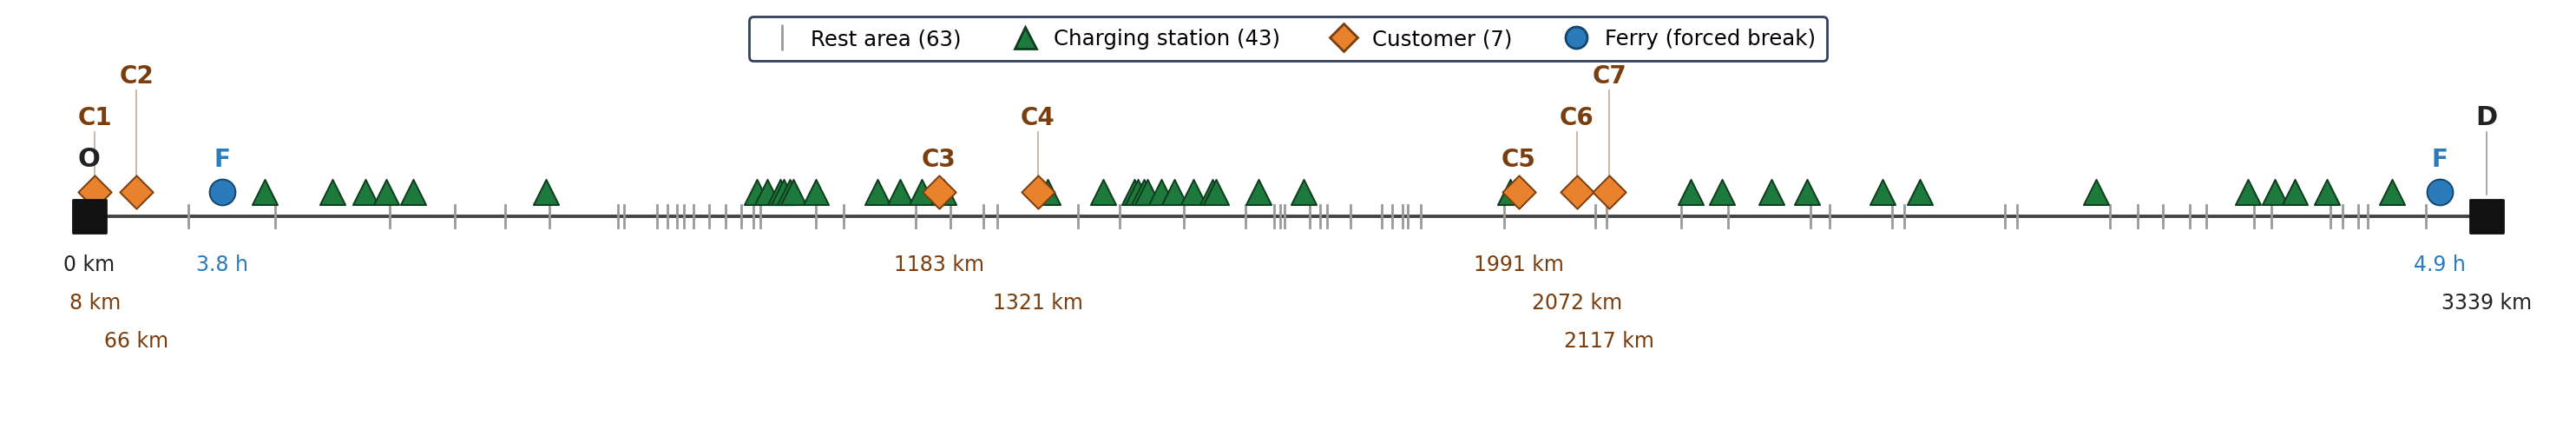
\includegraphics[width=\linewidth]{figures/real_route_strip.png}
    \caption{The real-life instance on the linear stop axis: origin and
    destination depot (O, D), seven anonymised customers (C1--C7), the
    charging set $\mathcal K$, the layby set $\mathcal L$, and the two ferry
    nodes (F) at which a break of the crossing duration is forced.  The sea
    crossings add no distance, which is why the outbound ferry sits only
    185\,km along the axis.}
    \label{fig:caseinstance}
\end{figure}
